\section{Experiments}

\begin{table*}[!t]
\centering
\caption{CoMani-Mod success rates.
Task IDs follow Table~\ref{tab:comani_tasks}.}
\label{tab:modifier_comparison}
\fontsize{7}{8.4}\selectfont
\setlength{\tabcolsep}{1.5pt}
\renewcommand{\arraystretch}{1.15}
\def\resultcolwidth{\dimexpr(\textwidth-2pt-1.7cm-42\tabcolsep-3\arrayrulewidth)/20\relax}
\begin{tabular}{p{1.7cm}|*{2}{>{\centering\arraybackslash}p{\resultcolwidth}}|*{12}{>{\centering\arraybackslash}p{\resultcolwidth}}|*{6}{>{\centering\arraybackslash}p{\resultcolwidth}}}
\noalign{\hrule height 1pt}
\multirow[c]{2}{*}{Method} & \multicolumn{2}{c|}{Mean SR} & \multicolumn{12}{c|}{ID SR} & \multicolumn{6}{c}{OOD SR} \\
\cline{2-21}
 & ID & OOD & 0 & 1 & 2 & 3 & 4 & 5 & 6 & 7 & 8 & 9 & 10 & 11 & 12 & 13 & 14 & 15 & 16 & 17 \\
\hline
% PointBridge sources: server 9996, point_bridge_points_custom0902-step_30000; ID libero_custom_0902-0912-025321-346811/result.json (103/360); OOD libero_custom_0902-0912-025322-202611/result.json (6/180). Verified against per-episode records and mapped through expr/task_id_mapping.json.
PointBridge & 28.6 & 3.3 & 0.0 & 36.7 & 60.0 & \textbf{100.0} & 0.0 & 0.0 & 83.3 & 63.3 & 0.0 & 0.0 & 0.0 & 0.0 & 20.0 & 0.0 & 0.0 & 0.0 & 0.0 & 0.0 \\
PointPolicy & 21.4 & 15.0 & 3.3 & 36.7 & 66.7 & 50.0 & 0.0 & 0.0 & 16.7 & 0.0 & 23.3 & 0.0 & 13.3 & 46.7 & 10.0 & 0.0 & 0.0 & 6.7 & 0.0 & 73.3 \\
DP3 & 73.6 & 57.2 & 73.3 & \textbf{100.0} & \textbf{100.0} & \textbf{100.0} & 53.3 & \textbf{100.0} & 0.0 & 80.0 & 80.0 & 86.7 & 26.7 & 83.3 & 86.7 & \textbf{63.3} & 60.0 & \textbf{93.3} & 16.7 & 23.3 \\
ACT & 20.0 & 7.2 & 33.3 & 20.0 & 6.7 & 23.3 & 13.3 & 56.7 & 10.0 & 3.3 & 63.3 & 0.0 & 0.0 & 10.0 & 30.0 & 0.0 & 0.0 & 13.3 & 0.0 & 0.0 \\
DP & 40.0 & 10.0 & 43.3 & 36.7 & 16.7 & 26.7 & 50.0 & 66.7 & 20.0 & 33.3 & 80.0 & 16.7 & 36.7 & 53.3 & 30.0 & 0.0 & 0.0 & 30.0 & 0.0 & 0.0 \\
$\pi_{0.5}$ & 91.1 & 48.3 & \textbf{100.0} & \textbf{100.0} & 56.7 & \textbf{100.0} & 73.3 & \textbf{100.0} & 96.7 & \textbf{83.3} & \textbf{100.0} & \textbf{100.0} & 83.3 & \textbf{100.0} & 80.0 & 33.3 & 6.7 & 80.0 & 6.7 & \textbf{83.3} \\
\hline
GraphPoint & \textbf{96.4} & \textbf{75.6} & \textbf{100.0} & \textbf{100.0} & \textbf{100.0} & 86.7 & \textbf{93.3} & \textbf{100.0} & \textbf{100.0} & 80.0 & \textbf{100.0} & \textbf{100.0} & \textbf{96.7} & \textbf{100.0} & \textbf{100.0} & \textbf{63.3} & \textbf{73.3} & 76.7 & \textbf{73.3} & 66.7 \\
\noalign{\hrule height 1pt}
\end{tabular}
\end{table*}

\begin{table*}[!t]
\centering
\caption{CoMani-Act action-consistent success rates (ACSR).
Task IDs follow Table~\ref{tab:comani_tasks}.}
\label{tab:action_comparison}
\fontsize{7}{8.4}\selectfont
\setlength{\tabcolsep}{1.5pt}
\renewcommand{\arraystretch}{1.15}
\def\resultcolwidth{\dimexpr(\textwidth-2pt-1.7cm-26\tabcolsep-3\arrayrulewidth)/12\relax}
\begin{tabular}{p{1.7cm}|*{2}{>{\centering\arraybackslash}p{\resultcolwidth}}|*{7}{>{\centering\arraybackslash}p{\resultcolwidth}}|*{3}{>{\centering\arraybackslash}p{\resultcolwidth}}}
\noalign{\hrule height 1pt}
\multirow[c]{2}{*}{Method} & \multicolumn{2}{c|}{Mean ACSR} & \multicolumn{7}{c|}{ID ACSR} & \multicolumn{3}{c}{OOD ACSR} \\
\cline{2-13}
 & ID & OOD & 0 & 1 & 2 & 3 & 4 & 5 & 6 & 7 & 8 & 9 \\
\hline
PointPolicy & 80.5 & 4.4 & \textbf{100.0} & 73.3 & 23.3 & \textbf{100.0} & \textbf{100.0} & 76.7 & 90.0 & 13.3 & 0.0 & 0.0 \\
DP3 & 83.3 & 60.0 & 80.0 & 93.3 & \textbf{96.7} & \textbf{100.0} & \textbf{100.0} & 86.7 & 26.7 & \textbf{80.0} & 0.0 & \textbf{100.0} \\
$\pi_{0.5}$ &  &  &  &  &  &  &  &  &  &  &  &  \\
\hline
GraphPoint & \textbf{90.5} & \textbf{64.4} & 50.0 & \textbf{100.0} & 83.3 & \textbf{100.0} & \textbf{100.0} & \textbf{100.0} & \textbf{100.0} & 26.7 & \textbf{76.7} & 90.0 \\
\noalign{\hrule height 1pt}
\end{tabular}
\end{table*}

% Defer the sequence and following ablation tables by one page.
\afterpage{\afterpage{
\begin{table*}[!t]
\centering
\caption{CoMani-Seq success rate (SR) and progress rate (PR).
Environment-based switching (ES) uses goal signals; self-switching (SS) uses predicted progress.
Mean groups by OOD count; task IDs follow Table~\ref{tab:comani_tasks}.}
\label{tab:sequence_comparison}
\fontsize{7}{8.4}\selectfont
\setlength{\tabcolsep}{1.5pt}
\renewcommand{\arraystretch}{1.15}
\def\resultcolwidth{\dimexpr(\textwidth-2pt-4.3cm-44\tabcolsep-11\arrayrulewidth)/20\relax}
\begin{tabular}{p{3.3cm}|>{\centering\arraybackslash}p{1.0cm}|*{9}{*{2}{>{\centering\arraybackslash}p{\resultcolwidth}}|}*{2}{>{\centering\arraybackslash}p{\resultcolwidth}}}
\noalign{\hrule height 1pt}
\multirow[c]{3}{*}{Method} & \multirow[c]{3}{*}{Switch} & \multicolumn{8}{c|}{Mean} & \multicolumn{4}{c|}{3 ID} & \multicolumn{4}{c|}{2 ID + 1 OOD} & \multicolumn{4}{c}{2/1 ID + 1/2 OOD} \\
\cline{3-22}
 & & \multicolumn{2}{c|}{All} & \multicolumn{2}{c|}{0 OOD} & \multicolumn{2}{c|}{1 OOD} & \multicolumn{2}{c|}{2 OOD} & \multicolumn{2}{c|}{0} & \multicolumn{2}{c|}{1} & \multicolumn{2}{c|}{2} & \multicolumn{2}{c|}{3} & \multicolumn{2}{c|}{4} & \multicolumn{2}{c}{5} \\
\cline{3-22}
 & & SR & PR & SR & PR & SR & PR & SR & PR & SR & PR & SR & PR & SR & PR & SR & PR & SR & PR & SR & PR \\
\hline
PointPolicy & ES & 0.0 & 0.0 & 0.0 & 0.0 & 0.0 & 0.0 & 0.0 & 0.0 & 0.0 & 0.0 & 0.0 & 0.0 & 0.0 & 0.0 & 0.0 & 0.0 & 0.0 & 0.0 & 0.0 & 0.0 \\
DP3 & ES & 0.0 & 11.1 & 0.0 & 16.7 & 0.0 & 11.1 & 0.0 & 0.0 & 0.0 & 26.7 & 0.0 & 6.7 & 0.0 & 30.0 & 0.0 & 3.3 & 0.0 & 0.0 & 0.0 & 0.0 \\
$\pi_{0.5}$ & ES & 0.0 & 25.0 & 0.0 & 28.3 & 0.0 & 26.7 & 0.0 & 13.3 & 0.0 & 33.3 & 0.0 & 23.3 & 0.0 & 33.3 & 0.0 & 33.3 & 0.0 & 13.3 & 0.0 & 13.3 \\
\hline
GraphPoint & ES & 51.7 & 79.4 & 75.0 & 95.0 & 50.0 & 81.1 & 10.0 & 43.3 & 60.0 & 90.0 & 90.0 & 100.0 & 30.0 & 76.7 & 30.0 & 70.0 & 90.0 & 96.7 & 10.0 & 43.3 \\
GraphPoint & SS & 38.3 & 78.3 & 65.0 & 90.0 & 26.7 & 77.8 & 20.0 & 56.7 & 90.0 & 96.7 & 40.0 & 83.3 & 20.0 & 76.7 & 10.0 & 73.3 & 50.0 & 83.3 & 20.0 & 56.7 \\
\noalign{\hrule height 1pt}
\end{tabular}
\end{table*}
\begin{table*}[!t]
\centering
\caption{CoMani-Mod ablation success rates.
Task IDs follow Table~\ref{tab:comani_tasks}.}
\label{tab:modifier_ablation}
\fontsize{7}{8.4}\selectfont
\setlength{\tabcolsep}{1.5pt}
\renewcommand{\arraystretch}{1.15}
\def\resultcolwidth{\dimexpr(\textwidth-2pt-3.0cm-42\tabcolsep-3\arrayrulewidth)/20\relax}
\begin{tabular}{p{3.0cm}|*{2}{>{\centering\arraybackslash}p{\resultcolwidth}}|*{12}{>{\centering\arraybackslash}p{\resultcolwidth}}|*{6}{>{\centering\arraybackslash}p{\resultcolwidth}}}
\noalign{\hrule height 1pt}
\multirow[c]{2}{*}{Variant} & \multicolumn{2}{c|}{Mean SR} & \multicolumn{12}{c|}{ID SR} & \multicolumn{6}{c}{OOD SR} \\
\cline{2-21}
 & ID & OOD & 0 & 1 & 2 & 3 & 4 & 5 & 6 & 7 & 8 & 9 & 10 & 11 & 12 & 13 & 14 & 15 & 16 & 17 \\
\hline
w/o RPC & 90.6 & 44.4 & \textbf{100.0} & 96.7 & \textbf{100.0} & \textbf{100.0} & 66.7 & 96.7 & 96.7 & 83.3 & 93.3 & \textbf{100.0} & 70.0 & 83.3 & 20.0 & \textbf{90.0} & \textbf{80.0} & 6.7 & 10.0 & 60.0 \\
Full connectivity & 95.3 & 63.9 & 96.7 & 96.7 & \textbf{100.0} & \textbf{100.0} & \textbf{100.0} & 83.3 & \textbf{100.0} & \textbf{86.7} & \textbf{100.0} & \textbf{100.0} & 80.0 & \textbf{100.0} & 66.7 & 86.7 & 70.0 & 50.0 & 36.7 & \textbf{73.3} \\
Merged entity point set & 82.8 & 27.8 & 93.3 & 96.7 & \textbf{100.0} & \textbf{100.0} & 93.3 & 26.7 & 83.3 & 56.7 & \textbf{100.0} & 96.7 & 50.0 & 96.7 & 60.0 & 0.0 & 36.7 & 3.3 & 3.3 & 63.3 \\
Absolute point coordinates & 92.5 & 25.0 & 90.0 & \textbf{100.0} & \textbf{100.0} & 96.7 & 86.7 & \textbf{100.0} & 96.7 & 46.7 & \textbf{100.0} & \textbf{100.0} & 93.3 & \textbf{100.0} & 3.3 & 63.3 & 3.3 & 6.7 & 6.7 & 66.7 \\
Delta-action output & 95.0 & 73.3 & 96.7 & \textbf{100.0} & \textbf{100.0} & \textbf{100.0} & \textbf{100.0} & 96.7 & 80.0 & \textbf{86.7} & \textbf{100.0} & \textbf{100.0} & 80.0 & \textbf{100.0} & 96.7 & 86.7 & 76.7 & \textbf{76.7} & 50.0 & 53.3 \\
\hline
GraphPoint & \textbf{96.4} & \textbf{75.6} & \textbf{100.0} & \textbf{100.0} & \textbf{100.0} & 86.7 & 93.3 & \textbf{100.0} & \textbf{100.0} & 80.0 & \textbf{100.0} & \textbf{100.0} & \textbf{96.7} & \textbf{100.0} & \textbf{100.0} & 63.3 & 73.3 & \textbf{76.7} & \textbf{73.3} & 66.7 \\
\noalign{\hrule height 1pt}
\end{tabular}
\end{table*}
}}

\begin{figure*}[!t]
\centering
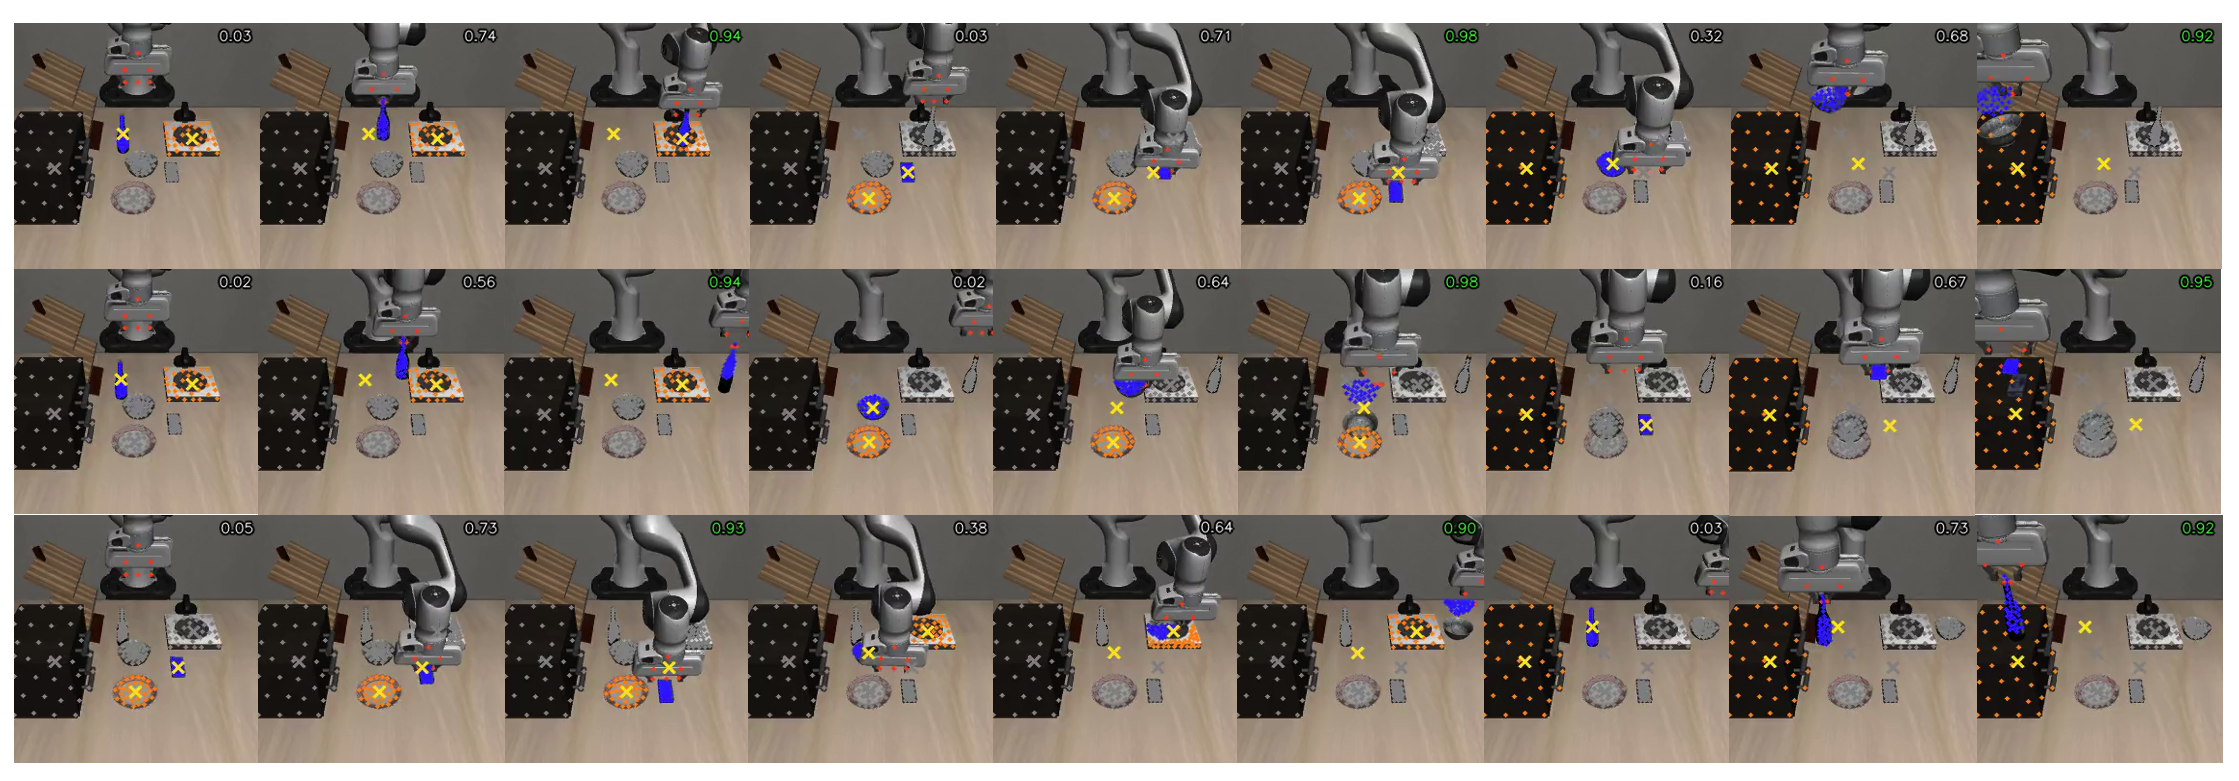
\includegraphics[width=\textwidth]{fig/vis.png}
\caption{Successful GraphPoint SS rollouts on CoMani-Seq.
Rows show sequences containing 0, 1, and 2 OOD subtasks, respectively, from top to bottom.
Each row proceeds from left to right, with 3 frames per subtask showing its start, execution, and completion.
Upper-right values show predicted subtask progress.
Apparent point-tracking mismatches are visualization artifacts, not actual tracking failures.}
\label{fig:sequence_rollouts}
\end{figure*}



\subsection{Experimental Setup}
\textbf{Baselines and adaptation.}
We compare GraphPoint with ACT~\cite{zhao2023act}, DP~\cite{chi2023dp}, DP3~\cite{ze2024dp3}, PointPolicy~\cite{haldar2025pp}, PointBridge~\cite{haldar2026pb}, and $\pi_{0.5}$~\cite{physicalintelligence2025pi05}.
ACT and DP use color images and robot state; DP3 uses scene point clouds and state. PointPolicy and PointBridge use LIBERO entity points and gripper-point supervision.
We adapt ACT, DP, DP3, and PointPolicy to multi-task instructions using frozen BGE embeddings of the full instruction, without role/action/modifier decomposition.
ACT projects this embedding into an additional Transformer encoder token; PointPolicy appends a projected language token to its point-token sequence.
DP and DP3 combine language and observation features through their existing FiLM conditioning paths.
PointBridge retains its native language-token pathway: frozen MiniLM sentence embeddings pass through a learned MLP and precede observation tokens in the causal Transformer.
$\pi_{0.5}$ retains its native image--text prefix conditioning and is fine-tuned with LoRA, without an added BGE encoder.
For CoMani-Seq, atomic policies are reused without sequence-level training, receiving the active subtask instruction under a shared ES protocol; GraphPoint is also evaluated with SS.

\textbf{Training and evaluation.}
All models are trained or fine-tuned on the first 10 demonstrations of each ID task for 30,000 steps with batch size 64 and AdamW; OOD tasks are excluded from training.
We evaluate at 20\,Hz over 30 trials per task on CoMani-Mod and CoMani-Act, and 10 trials per sequence on CoMani-Seq, using the splits in Sec.~\ref{sec:benchmark}.
Sequence rollouts allow 1,500 action steps after 30 settling steps and share initial-state indices across methods.
We use the suite-specific metrics defined in Sec.~\ref{sec:benchmark}: SR for CoMani-Mod, ACSR for CoMani-Act, and SR/PR for CoMani-Seq.
Tables report task means and ID/OOD aggregates, with unfinished evaluations left blank.

We evaluate modifier and action composition, sequential skill reuse, and component contributions.
% IMPORTANT: Map code IDs through expr/task_id_mapping.json before entering results.
% Existing numeric result columns retain their original task correspondence.
% Sources: expr/1.csv (Modifier comparison and ablations), expr/2.csv (Action).
% PI05 CoMani-Mod source: openpi/data/libero/pi05_custom0902_step29999/{id,ood}, 30 trials/task.
% Aggregate rates are copied from CSV SR-ID/SR-OOD, avoiding re-averaging rounded task percentages.
% Pending baseline cells must be filled from completed evaluations, not inferred from expected rankings.

\subsection{Can GraphPoint Generalize Across Modifiers?}
Table~\ref{tab:modifier_comparison} shows 96.4\% ID and 75.6\% OOD success for GraphPoint, exceeding the strongest baselines, $\pi_{0.5}$ on ID and DP3 on OOD, by 5.3 and 18.3 percentage points.
ACT, DP, PointPolicy, and PointBridge have low ID success, so their OOD results reflect limitations in both task acquisition and generalization.
GraphPoint achieves at least 63.3\% on every OOD task, compared with DP3's 16.7--93.3\% range.
For wine-bottle placement on the cabinet, it reaches 73.3\% versus 16.7\%; however, DP3 leads on placing cream cheese right of the cabinet (93.3\% versus 76.7\%).
These results support broader held-out relation coverage, while leaving an ID--OOD gap.

\subsection{Can GraphPoint Generalize Across Actions?}
Table~\ref{tab:action_comparison} evaluates action composition on CoMani-Act; $\pi_{0.5}$ results remain pending. PointPolicy reaches 80.5\% ID and 4.4\% OOD ACSR.
GraphPoint reaches 90.5\% ID and 64.4\% OOD ACSR, compared with 83.3\% and 60.0\% for DP3.
The modest average OOD advantage masks substantial differences across held-out tasks.
GraphPoint transfers rotation from the stove knob to cream cheese with 76.7\% ACSR, while DP3 obtains 0\%.
GraphPoint trails DP3 on putting cream cheese to the right of the stove, with 26.7\% versus 80.0\%, and on sweeping the bowl to the right of the plate, with 90.0\% versus 100.0\%.
Thus, these results support cross-entity rotation transfer but do not establish a uniform advantage across action combinations.
% PointPolicy Act sources: point_policy_custom0904-step_30000/libero_custom_0904-0913-131340-809426 and libero_custom_0904-0913-131421-638036; 300 unique completed episodes; author action review excludes 13 terminal successes for code task 3 (paper task 7), leaving 4/30. Raw final_goals records are preserved. Paper order: 0,1,2,5,7,8,9,3,4,6.
% The author confirmed that the reported CoMani-Act rates include action-process checks.

\subsection{Can GraphPoint Compose Atomic Skills?}
Table~\ref{tab:sequence_comparison} evaluates atomic policies on six three-step sequences without sequence-level training.
GraphPoint achieves 51.7\% SR and 79.4\% PR with ES, versus 38.3\% and 78.3\% with SS using patient/target progress summaries.
The 13.33-point SR drop despite a 1.11-point PR decrease shows that similar partial progress does not guarantee full completion.
With ES, PointPolicy, DP3, and $\pi_{0.5}$ all obtain 0\% SR, with PR of 0.0\%, 11.1\%, and 25.0\%, respectively.
GraphPoint's ES success decreases from 75.0\% with no OOD subtasks to 50.0\% with one and 10.0\% with two.
In the final task pair, changing only bowl-on-stove to the OOD bowl-right-of-stove subtask reduces SR from 90.0\% to 10.0\%, illustrating how atomic generalization limits sequence completion.
Fig.~\ref{fig:sequence_rollouts} shows successful SS executions across all three OOD counts and their entity/progress transitions.

% Including actor summaries (A+P+T) yields 41.67\% SR and 74.44\% PR under self-switching, compared with 38.33\% and 78.33\% for P+T. The mixed changes do not establish a consistent advantage for either progress-head input on these 60 trials.
% Seq paper IDs 0,1,2,3,4,5 map to code IDs 2,3,0,1,4,5.
% Use expr/task_id_mapping.json when entering results; display SR and PR as percentages to 1 decimal.
% Completed Seq sources: DP3 oracle 0913-045046-444735; GP oracle 0913-032319-902357; GP predicted 0913-033203-484464.
% PointPolicy Seq source: point_policy_custom0902-step_30000/libero_custom_0906-oracle-0913-093609-073005/result.json (60/60 episodes; verified against dualgpu0/1 partitions and per-episode records).
% PI05 Seq source: custom0902_id10ep-29999/libero_custom_0906-oracle-0913-085835-851951/result.json (60/60 episodes).
% A+P+T Seq source: allprogress predicted 0913-045808-238820 (60/60 episodes).
% Hidden row (preserved values): GraphPoint (A+P+T) & SS & 41.7 & 74.4 & 85.0 & 93.3 & 16.7 & 64.4 & 30.0 & 66.7 & 90.0 & 100.0 & 80.0 & 86.7 & 20.0 & 63.3 & 10.0 & 63.3 & 20.0 & 66.7 & 30.0 & 66.7 \\
% SR uses result.success_rate; PR uses result.progress_rate (not server_success_rate).

\subsection{Which Components Matter?}
Table~\ref{tab:modifier_ablation} examines GraphPoint variants on CoMani-Mod.
We remove RPC, replace chain attention with full connectivity, merge the entity graph into a single point set, use absolute point coordinates, or predict Cartesian delta actions instead of point trajectories.

\textbf{Geometry and graph structure.}
Removing RPC reduces OOD success by 31.1 percentage points, compared with a 5.8-point ID decrease, consistent with its intended role in reducing dependence on detailed training geometry.
Full graph connectivity retains 95.3\% ID success but lowers OOD success to 63.9\%, supporting patient-mediated interaction as a useful inductive bias.
Merging all entity points yields 27.8\% OOD success despite retaining 12 summary tokens in total.
This variant jointly removes role embeddings, separate local entity groups, and chain connectivity, and reads shared summaries for progress; it therefore tests the structured encoder as a whole rather than any single component.

\textbf{Coordinate and output representations.}
Using absolute point coordinates lowers OOD success to 25.0\% while retaining 92.5\% ID success, indicating that relative geometry is particularly useful for held-out combinations.
Replacing point trajectories with Cartesian delta actions gives 95.0\% ID and 73.3\% OOD success, close to the full model.
The observed gains are therefore more pronounced for relative coordinates, geometric augmentation, and role structure than for point output alone.
These comparisons describe the reported checkpoint evaluations; repeated-training estimates are needed to assess the reliability of small differences.
